\begin{figure*}[hbtp]
  \centering
  % \includegraphics[width=0.44\linewidth]{out/deletions-runtime-key.pdf}
  \subfigure[Overall result]{
    \label{fig:deletions-runtime--mean}
    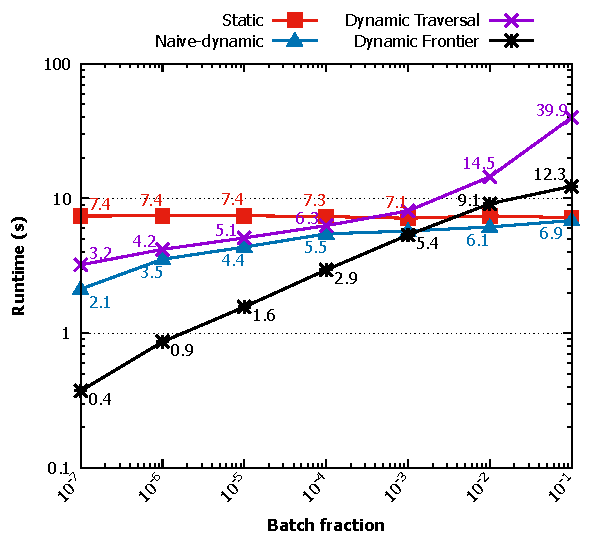
\includegraphics[width=0.38\linewidth]{out/deletions-runtime-mean.pdf}
  }
  \subfigure[Results on each graph]{
    \label{fig:deletions-runtime--all}
    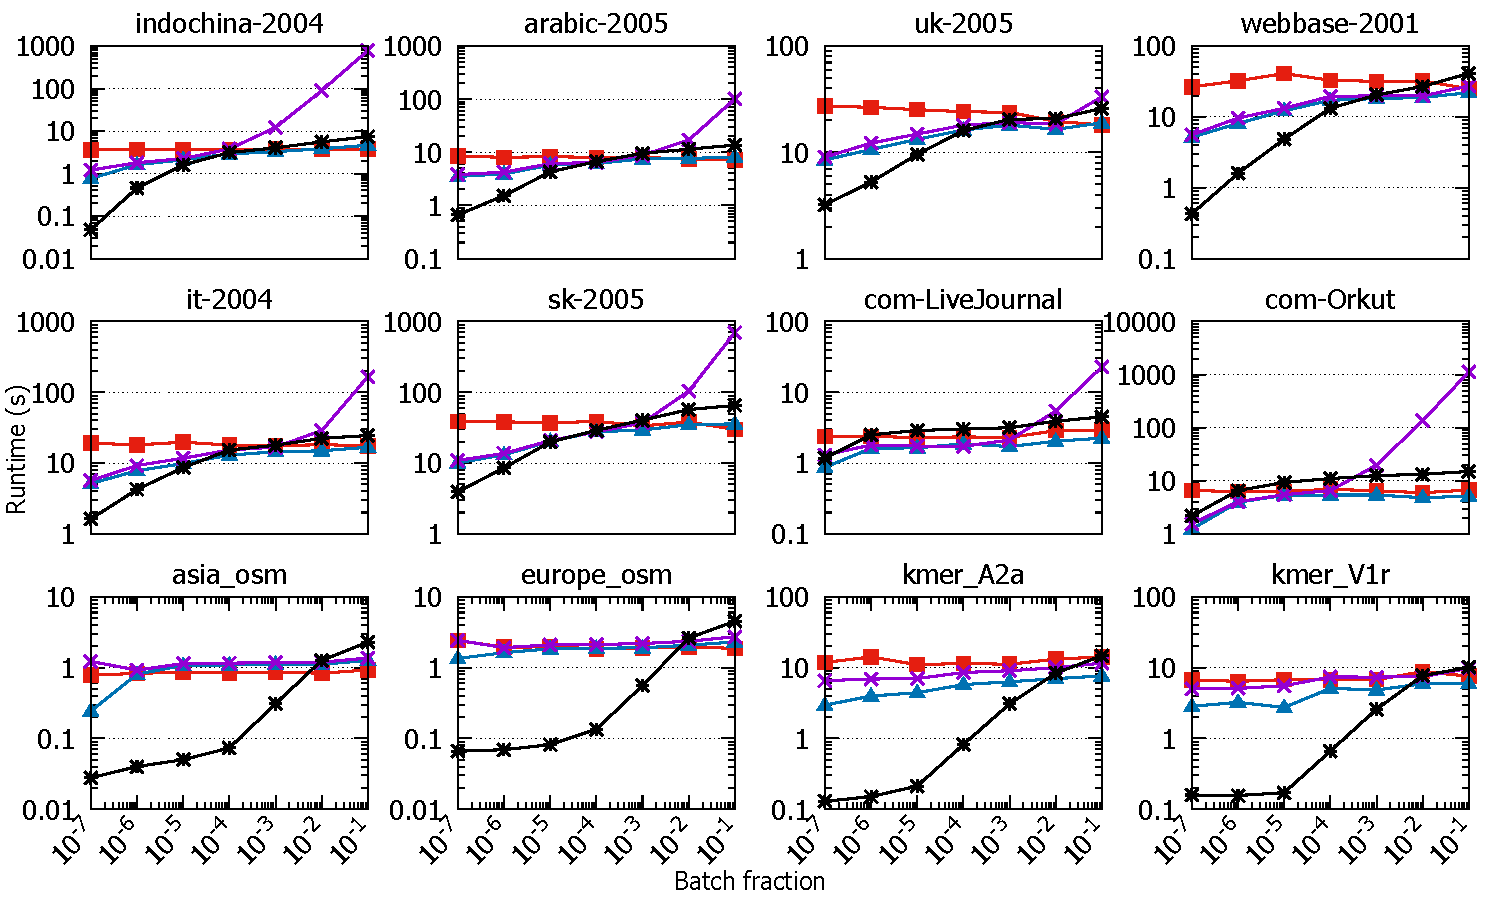
\includegraphics[width=0.58\linewidth]{out/deletions-runtime-all.pdf}
  } \\[-1ex]
  \caption{Runtime (logarithmic scale) of \textit{Static}, \textit{Naive-dynamic}, \textit{Dynamic Traversal}, and \textit{Dynamic Frontier} PageRank with batch updates, consisting purely of edge deletions, increasing from $10^{-7} |E|$ to $0.1 |E|$, in multiples of $10$ (logarithmic scale). The figure on the right illustrates the runtime of each approach for individual graphs in the dataset, while the figure of the left presents overall runtimes (using geometric mean for consistent scaling across graphs).}
  \label{fig:deletions-runtime}
\end{figure*}
